%
%  Vincent Yannello
%
\documentclass[12pt,fullpage]{article}
\usepackage{fullpage}
\usepackage{psfrag}                                          % LaTeX graphics tool
\usepackage{pslatex}                                         % avoids the default cmr font
\usepackage{graphicx}                                        % graphics package 
\usepackage{epsfig}                                          % figures
\usepackage{hyperref}
\usepackage{color}

\begin{document}

\noindent
{\bf Hyperexponential distribution} (from \color{blue}\url{http://www.math.wm.edu/~leemis/chart/UDR/UDR.html}\color{black})

\noindent
The shorthand $X \sim {\rm hyperexponential}(\vec\alpha,\, \vec p)$ is used to indicate that the
random variable $X$ has the hyperexponential distribution with parameters $\vec\alpha$ and $\vec p$.
A hyperexponential random variable $X$ with parameters $\vec \alpha$ and $\vec p$ has probability density function 
$$
f(x) = \displaystyle\sum_{i \, = \, 1} ^ {n} \frac{p_i} {\alpha_{\kern 0.08 em i}} e ^ {-x / \alpha_{\kern 0.08 em i}} \qquad \qquad x > 0
$$
for all $\alpha_{\kern 0.08 em i}, p_i > 0$ such that $\sum_{i \, = \, 1} ^ n p_i = 1$.
The probability density function for $\vec \alpha = (0.25, \, 0.5, \, 1)$ and $\vec p = (0.5, \, 0.25, \, 0.25)$ is illustrated below.

\begin{figure}[h!]
\begin{center}
\psfrag{labf}{$f(x)$}
\psfrag{labx}{$x$}
\includegraphics[width=3.2in]{HyperexponentialPlot.ps}
\end{center}
\end{figure}

\noindent
The cumulative distribution function on the support of $X$ is
$$
F(x) = P(X \leq x) = 1 - \displaystyle \sum_{i \, = \, 1} ^ {n} p_i \kern 0.08 em e ^ {-x / \alpha_{\kern 0.08 em i}} \qquad \qquad x > 0.
$$
The survivor function on the support of $X$ is
$$
S(x) = P(X \leq x) = \displaystyle \sum_{i \, = \, 1} ^ {n} p_i \kern 0.08 em e ^ {-x / \alpha_{\kern 0.08 em i}} \qquad \qquad x > 0.
$$
The hazard function on the support of $X$ is
$$
h(x) = \frac{f(x)}{S((x)} = \frac{\sum_{i \, = \, 1} ^ {n} \frac{p_i} {\alpha_{\kern 0.08 em i}} e ^ {-x / \alpha_{\kern 0.08 em i}} }
       {\sum_{i \, = \, 1} ^ {n} p_i \kern 0.08 em e ^ {-x / \alpha_{\kern 0.08 em i}}} \qquad \qquad x > 0.
$$
The inverse distribution function and characteristic function are both mathematically intractable. \\
\\
\noindent
The moment generating function over the support of $X$ is
$$
M(t) = E[e ^ {\kern 0.08 em tX}] = \displaystyle \sum_{i \, = \, 1} ^ n \frac{p_i} {1 - \alpha_{\kern 0.08 em i} \kern 0.08 em t} \qquad \qquad |t| < \frac{1}{\min_{j} \kern 0.08 em \alpha_j}.
$$
\\
The population mean of $X$ is
$$
E[X] = \displaystyle \sum_{i \, = \, 1} ^ n p_i \kern 0.08 em \alpha_{\kern 0.08 em i}. \qquad \qquad 
$$
The population skewness and kurtosis of $X$ are all mathematically intractable.

\vspace{0.1in}

\noindent
{\bf APPL verification:}
The APPL statements
\begin{verbatim}
X := HyperExponentialRV([0.1, 0.3, 0.6], [alpha1, alpha2, alpha3]);
CDF(X);
SF(X);
Mean(X);
Variance(X);
Skewness(X);
Kurtosis(X);
MGF(X);
\end{verbatim}
verify the population mean, variance, skewness, kurtosis, and moment generating function
for the special case of $n=3$ and $\vec p = (0.1,\, 0.3,\, 0.6)$.

\end{document}
